\chapter{Stworzony model zjawiska}

Niniejszy rozdział opisuje szczegółowo kolejne kroki oraz wykorzystane algorytmy niezbędne do uzyskania efektu końcowego.

%---------------------------------------------------------------------------

\section{Opracowanie danych topograficznych}
\subsection{Format .las}
Na początkowym etapie pracy otrzymano pliki w formacie .las - każdy z nich reprezentujący ukształtowanie terenu wybranego obszaru. 

Format .las został stworzony do przechowywania zbioru punktów w przestrzeni trójwymiarowej (ang. point cloud), otrzymanych przy pomocy metody Lidar, która polega na oświetlaniu wybranych punktów na powierzchni Ziemi laserem i zapisie jego odbicia przy pomocy sensorów. Dzięki tej metodzie powstają mapy o wysokiej rozdzielczości, stosowane w naukach o Ziemi (źródło: angielska wiki). 

Otrzymane pliki zawierały średnio około 11 milionów punktów, przy czym każdy z nich reprezentował powierzchnię około 4 km$^2$.

\begin{figure}[h]
	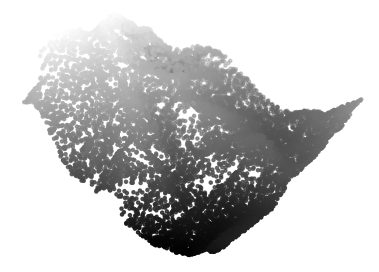
\includegraphics[width=8cm]{las_example}
	\centering
	\caption{Uproszczona wizualizacja zbioru punktów z pliku .las przy użyciu biblioteki matplotlib}
\end{figure}

\subsection{Wybór cech}
Jak wspomniano już wcześniej, do oszacowania ryzyka lawinowego konieczne jest posiadanie danych dotyczących cech terenu. Bazując na pracy pani Izabeli Woszczak, skupiono się na obliczeniu taki cech, jak:
\begin{itemize}
	\item forma terenu (skupiono się na żlebach);
	\item ekspozycja słoneczna;
	\item nachylenie powierzchni;
	\item piętro;
	\item wysokość.
\end{itemize}

\subsection{Triangulacja Delaunaya}
Sam zbiór punktów nie oferuje możliwości łatwego obliczania wyżej wymienionych cech, dlatego zastosowano uproszczenie powierzchni terenu przy pomocy triangulacji Delaunaya.

Jest to algorytm, który na podstawie zbioru punktów tworzy zbiór trójkątów, gdzie wierzchołki każdego trójkąta stanowią owe punkty. Własnością algorytmu jest, że maksymalizuje on najmniejsze z katów w powstałych trójkątach, unikając tzw. sliver triangles.


\begin{figure}[h]
	\centering
	\begin{minipage}{.5\textwidth}
		\centering
		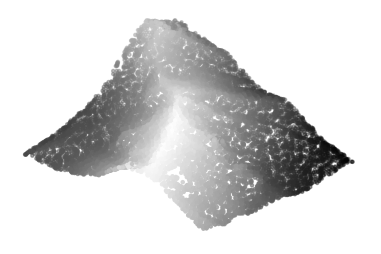
\includegraphics[width=.6\linewidth]{no_delaunay}
		\captionof{figure}{Obszar przedstawiony jako zbiór punktów}
		\label{fig:test1}
	\end{minipage}%
	\begin{minipage}{.5\textwidth}
		\centering
		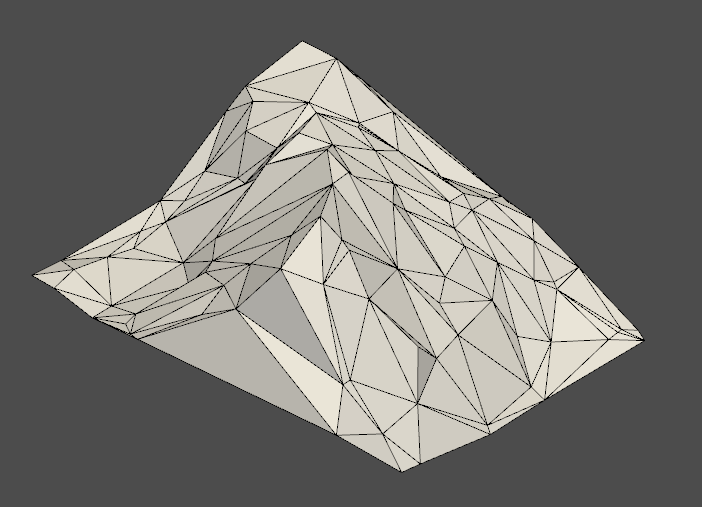
\includegraphics[width=.6\linewidth]{delaunay}
		\captionof{figure}{Ten samo obszar poddany triangulacji}
		\label{fig:test2}
	\end{minipage}
\end{figure}
Tutaj możesz dodać potem jak dokładniej policzyłeś ostatenie te nachylenia, bo szczerze mówiąc nie zaglądałem do tego jakoś szczegółowo xD
\clearpage

%---------------------------------------------------------------------------

\section{Opracowanie danych pogodowych}
\label{sec:kompilacja}


Dane pogodowe są kolejnymi kluczowymi danymi potrzebnymi do przewidzenia wystąpienia lawiny na danym obszarze. Wyodrębnione zostały 4 najważniejsze cechy wpływające na występowanie lawiny.
\begin{enumerate}
	\item Grubość pokrywy śnieżnej
	\item Zmiany temperatury
	\item Opad deszczu
	\item Prędkość wiatru
\end{enumerate}
\subsection{Progi pogodowe}
Na podstawie słowackiej strony \url{http://www.laviny.sk} przyjęliśmy następujące progi dla poszczególnych cech.
\subsubsection{Grubość pokrywy śnieżnej}
Dolny próg wysokości pokrywy śnieżnej niezbędnej do wystąpienia lawiny obraliśmy jako 20 centymetrów. Ze względu na bardzo ograniczone dane o zalegającej pokrywie śnieżnej na chwilę obecną te cechę jako spełnioną uznajemy w momencie, gdy w ostatnich 48 godzinach opad śniegu przekroczył próg 200mm.
\subsubsection{Zmiany temperatury}
Temperatura, zwłaszcza w okresie wczesnej lub późnej zimy, często ulega zmianom w okolicach 0\degree C.
Pokrywa śnieżna może nadtopnieć w dodatniej temperaturze i następnie zamarznąć, tworząc śliską warstwę która, kiedy ma na sobie warstwę śniegu, może w wysokim stopniu sprzyjać osunięciu się pokrywy i spowodowaniu lawiny. Z tego powodu przyjmujemy iż kiedy w ciągu ostatnich 48 godzin temperatura ulegnie zmianie z ujemnej na dodatnią, i do tego średnia temperatura jest powyżej zera, uznajemy tą cechę jako zwiąkszającą zagrożenie lawiną.
\subsubsection{Opad deszczu}
Nie ma podanych konkretnych wartości co do opadów deszczu, jedynym punktem odniesienia jest to iż opad musi być intensywny żeby przyczynił sie do powstania lawiny. Z tego powodu przyjęliśmy iż jeżeli w ciągu ostatnich 48 godzin wystąpił opad o minimalnej intensywności 10mm/h to ta cecha jest uznawana za spełnioną.
\subsubsection{Prędkość wiatru}
Jeżeli w ciągu ostatnich 48 godzin wystąpił wiatr o minimalnej prędkości 13m/s to tą cechę uznajemy jako zwiększającą zagrożenie lawiną.

\subsection{Pobieranie danych pogodowych}
Do pobrania danych pogodowych skorzystaliśmy z Open Weather Map API umożliwiającego łatwe i szybkie pobranie danych pogodowych.




%---------------------------------------------------------------------------

\section{Narzędzia}
\label{sec:narzedzia}


%---------------------------------------------------------------------------

\section{Przygotowanie dokumentu}
\label{sec:przygotowanieDokumentu}

Plik źródłowy \LaTeX a jest zwykłym plikiem tekstowym. Przygotowując plik
źródłowy warto wiedzieć o kilku szczegółach:

\begin{itemize}
\item
Poszczególne słowa oddzielamy spacjami, przy czym ilość spacji nie ma znaczenia.
Po kompilacji wielokrotne spacje i tak będą wyglądały jak pojedyncza spacja.
Aby uzyskać {\em twardą spację}, zamiast znaku spacji należy użyć znaku {\em
tyldy}.

\item
Znakiem końca akapitu jest pusta linia (ilość pusty linii nie ma znaczenia), a
nie znaki przejścia do nowej linii.

\item
\LaTeX~sam formatuje tekst. \textbf{Nie starajmy się go poprawiać}, chyba, że
naprawdę wiemy co robimy.
\end{itemize} 


